\section*{Zielsetzung}
Der Versuch soll überprüfen, ob die im Dulong-Petit Gesetz %präposition, petitsche
angesprochenen Oszillationen der Atome einer klassischen Beschreibung genügt, %kein satzzeichen nach atome
oder ob die Quantenmechanik benötigt wird. %ausdruck


\section{Theorie}

\subsection{Definition der spezifischen Wärmekapazität}

Findet an einem Körper eine Temperaturänderung $\Delta T$ statt, ohne dass an ihm  %dass
Arbeit verrichtet wird, so kommt es zu einer Wärmeauf- bzw. abnahme $\Delta Q$. %komma zwischen haupt und nebensatz, Wärmeauf- bzw. abnahme
Mit dem ersten Hauptsatz der Thermodynamik ergibt sich der Zusammenhang %ohne dann

\begin{equation*}
\Delta Q=m c \Delta T.
\end{equation*}

Dabei sei $m$ die Masse und $c$ die Wärmekapazität
des Körpers.
Bezieht man diese auf eine Masseneinheit,
so wird $c$ als spezifische Wärmekapazität bezeichnet.
 %was meinst du damit? %

Des Weiteren gibt die Molwärme $C$
an, wie viel Wärmemenge $\map{d}Q$ benötigt wird, %ausdruck %
um ein Mol (eines beliebigen Stoffes) um $\map{d}T$ zu erwärmen.

Dabei hängt der Betrag der Molwärme davon ab, unter welchen Bedingungen
die Temperaturänderung hervor gerufens wird.
Hierbei wird zwischen der spezifischen Wärmekapazität bei konstantem
Volumen $C_{V}$ und bei konstantem Druck $C_{p}$ unterschieden.
Die Größe $C_{V}$ ist gegeben durch: %ist gegeben

\begin{equation}
\label{eq:molwarme}
C_V=\left(\frac{\map{d}U}{\map{d}T}\right)_V
\end{equation}


\subsection{Dulong-Petit-Gesetz}

Das Dulong-Petit-Gesetz sagt aus, dass die Atomwärme (im festem Aggregatzustand) bei %besser einheitlich.. petit gesetz oder petitsche gesetz
konstantem Volumen unabhängig von den chemischen Eigenschaften eines Elementes
und gleich $3R$ ist. %wieso sei?
Man bezeichnet $R$ als die allgemeine Gaskonstante. %vielleicht zahlenwert aufführen, keiner im Protokoll angegeben
Das Gesetz führt die makroskopischen thermodynamischen Phänomene
auf zufällige mikroskopischen Bewegungen der Atome zurück. %ausdruck
Das Dulong-Petit-Gesetz wird zum Teil aus dem %aus dem sogenannten
sogenannten Äquipartitionstheorem hergeleitet.
Das Theorem gibt Rückschlüsse auf die kinetische Energie eines Atoms %atoms
im thermischen Gleichgewicht, durch:

\begin{equation*}
\left< E_{kin} \right>=\frac{1}{2}kT
\end{equation*}

Mit diesem und weiteren Zusammenhängen folgt für die innere Energie $U$ %weiteren
einer Gitterstruktur mit drei Freiheitsgraden:

\begin{equation*}
\left< U_{fest} \right> = 3 \left< U \right>=3RT \quad \Rightarrow \quad C_{V}\overset{\eqref{eq:molwarme}}{=}3R
\end{equation*}

\subsection{Quantenmechanische Betrachtung}
Bei der quantenmechanischen Betrachtung wird angenommen,
dass die oszillierenden Atome nur quantisierte Energiezustände $\Delta u=n\hbar \omega \quad n\in\mathbb{N}$
annehmen können.
Unter Zuhilfenahme der Boltzmann-Verteilung kann dann auf den Zusammenhang  %unter
\begin{equation}
\label{eq:quant}
\left< U_{qm} \right> =\frac{3N_L \hbar \omega}{\exp\left(\hbar \frac{\omega}{k} T\right) -1}
\end{equation}

geschlossen werden. Dieser gilt für Bewegungen mit drei Freiheitsgraden.
Die Konstante $N_L = \SI{6.02e23}{\per\mol}$ wird als Loschmidtsche Zahl bezeichnet.
Für $T\to\infty$ läuft \eqref{eq:quant} gegen den aus der klassischen Physik bekannten Wert %ohne kommas
$3RT$.

\subsection{Bestimmung der spezifischen Wärmekapazität}
Da eine experimentelle Bestimmung der spezifischen Wärmekapazität
bei konstanten Volumen $C_V$ kaum möglich ist, %komma
bestimmt man stattdessen die Wärmekapazität bei konstanten Druck $C_P$. %bestimmt man
Beide Größen können durch den Zusammenhang %können

\begin{equation}
\label{eq:umrechnung_cp_cv}
C_P-C_V=9\alpha^2\kappa V_0 T \quad \text{mit} \, \kappa=V\left(\frac{\partial p}{\partial V}\right)_T
\end{equation}

ineinander umgerechnet werden.
Hierbei ist $\alpha$ ein linearer Ausdehnungskoeffizient, $\kappa$ das Kompressionsmodul und %ist
$V_0$ das Molvolumen.

Die Bestimmung erfolgt mithilfe eines Kalorimeters,
eines rohrförmigen Probekörpers mit der Masse $m_k$ und der Temperatur %eines,
$T_k$. Zusätzlich gibt es ein mit Wasser gefülltes Gefäß.
Das Wasser besitzt die Masse $m_w$ und die Temperatur $T_w$.
Nach Eintauchen des Körpers stellt sich im Gefäß die
Mischtemperatur $T_w$ ein.
Es ergibt sich folgende Abhängigkeit:

\begin{equation*}
\label{eq:zusammenhang_ck}
c_k=\frac{\left(c_wm_w+c_gm_g\right)\left(T_m-T_w\right)}{m_k\left(T_k-T_m\right)}
\end{equation*}

Die Wärmekapazität des Kalorimeters wird druch $c_gm_g$ dargestellt. %kalori
In einer weiteren Messung wird diese bestimmt. %in
Bei dieser werden zwei Wassermengen mit $m_x$ und $m_y$ und den
dazugehörigen Temperaturen $T_x$ und $T_y$ miteinander vermischt.
Mit der sich einstellenden Temperatur $T_M$ kann dann
durch den Zusammenhang:
\begin{equation}
\label{eq:zusammenhang_cgmg}
c_gm_g=\frac{c_wc_y\left(T_y-T_M\right)-c_wm_x\left(T_M-T_x\right)}{\left(T_M-T_x\right)}
\end{equation}
auf die Wärmekapazität geschlossen werden.

\subsection{Thermoelemente und ihre Funktionsweise} %Skizze
\begin{figure}
  \centering
  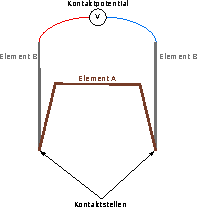
\includegraphics[width=0.45\textwidth]{bilder/thermoelement.pdf}
  \caption{Schematische Darstellung eines Thermoelements}
  \label{fig:thermo}
\end{figure}
Ein schematischer Aufbau eines Thermoelements ist in  Darstellung \ref{fig:thermo} %ausdruck
abgebildet.
Da ein Thermoelement eine hohe Einstellungsgeschwindigkeit besitzt,
wird es genutzt um schnell ändernde Temperatur zu messen. %ausdruck, haupt und nebensatz durch koomma trennen
Es besteht aus zwei Metallen, die sich jeweils durch
verschiedene Wärmeleitkoeffizienten auszeichnen.
Am Ende des Thermoelementes befindet sich ein Punkt an dem sich
beide Elemente berühren. Dieser Punkt wird als Berührungspunkt
bezeichnet.
Ein Thermoelement besitzt zwei Berührungsstellen.
Diese messen jeweils unterschiedliche Temperaturen $T_1$ und $T_2$.
Herrscht eine Temperaturdifferenz zwischen $T_1$ und $T_2$, so
stellt sich zwischen den Kontaktstellen ein Kontaktpotential %potential
ein.
Durch Messung der Spannung kann anschließend auf
Temperaturdifferenz geschlossen werden. %differenz
